\section{Algoritmen}
\subsection{Algemene uitleg}
De manier van aanpak werd dus veranderd. In plaats van een border langsheen de rand van het scherm te creëren is geopteerd geweest om de diagonalen te verbinden (een groene en een blauwe) en op het snijpunt wordt een lichtblauwe bol weergegeven \ref{fig:screen}. Door deze aanpassing wordt het makkelijker om te achterhalen tot welk island een los deel scherm behoort. De voorwaarde die we momenteel opleggen om een scherm te kunnen detecteren is dat twee aanliggende hoeken en het middelpunt zichtbaar zijn. Achter het kruis wordt nog steeds de barcode geplaatst om de schermen te identificeren.
Een offset werd toegevoegd tijdens het vormen van de islands omdat zo de ruis verwijderd wordt rond de overgangen van de achtergrondkleuren.Hieronder volgt een opsomming van de methoden die toegepast worden op de input image in chronologische volgorde.
\center
\begin{figure} [h]
	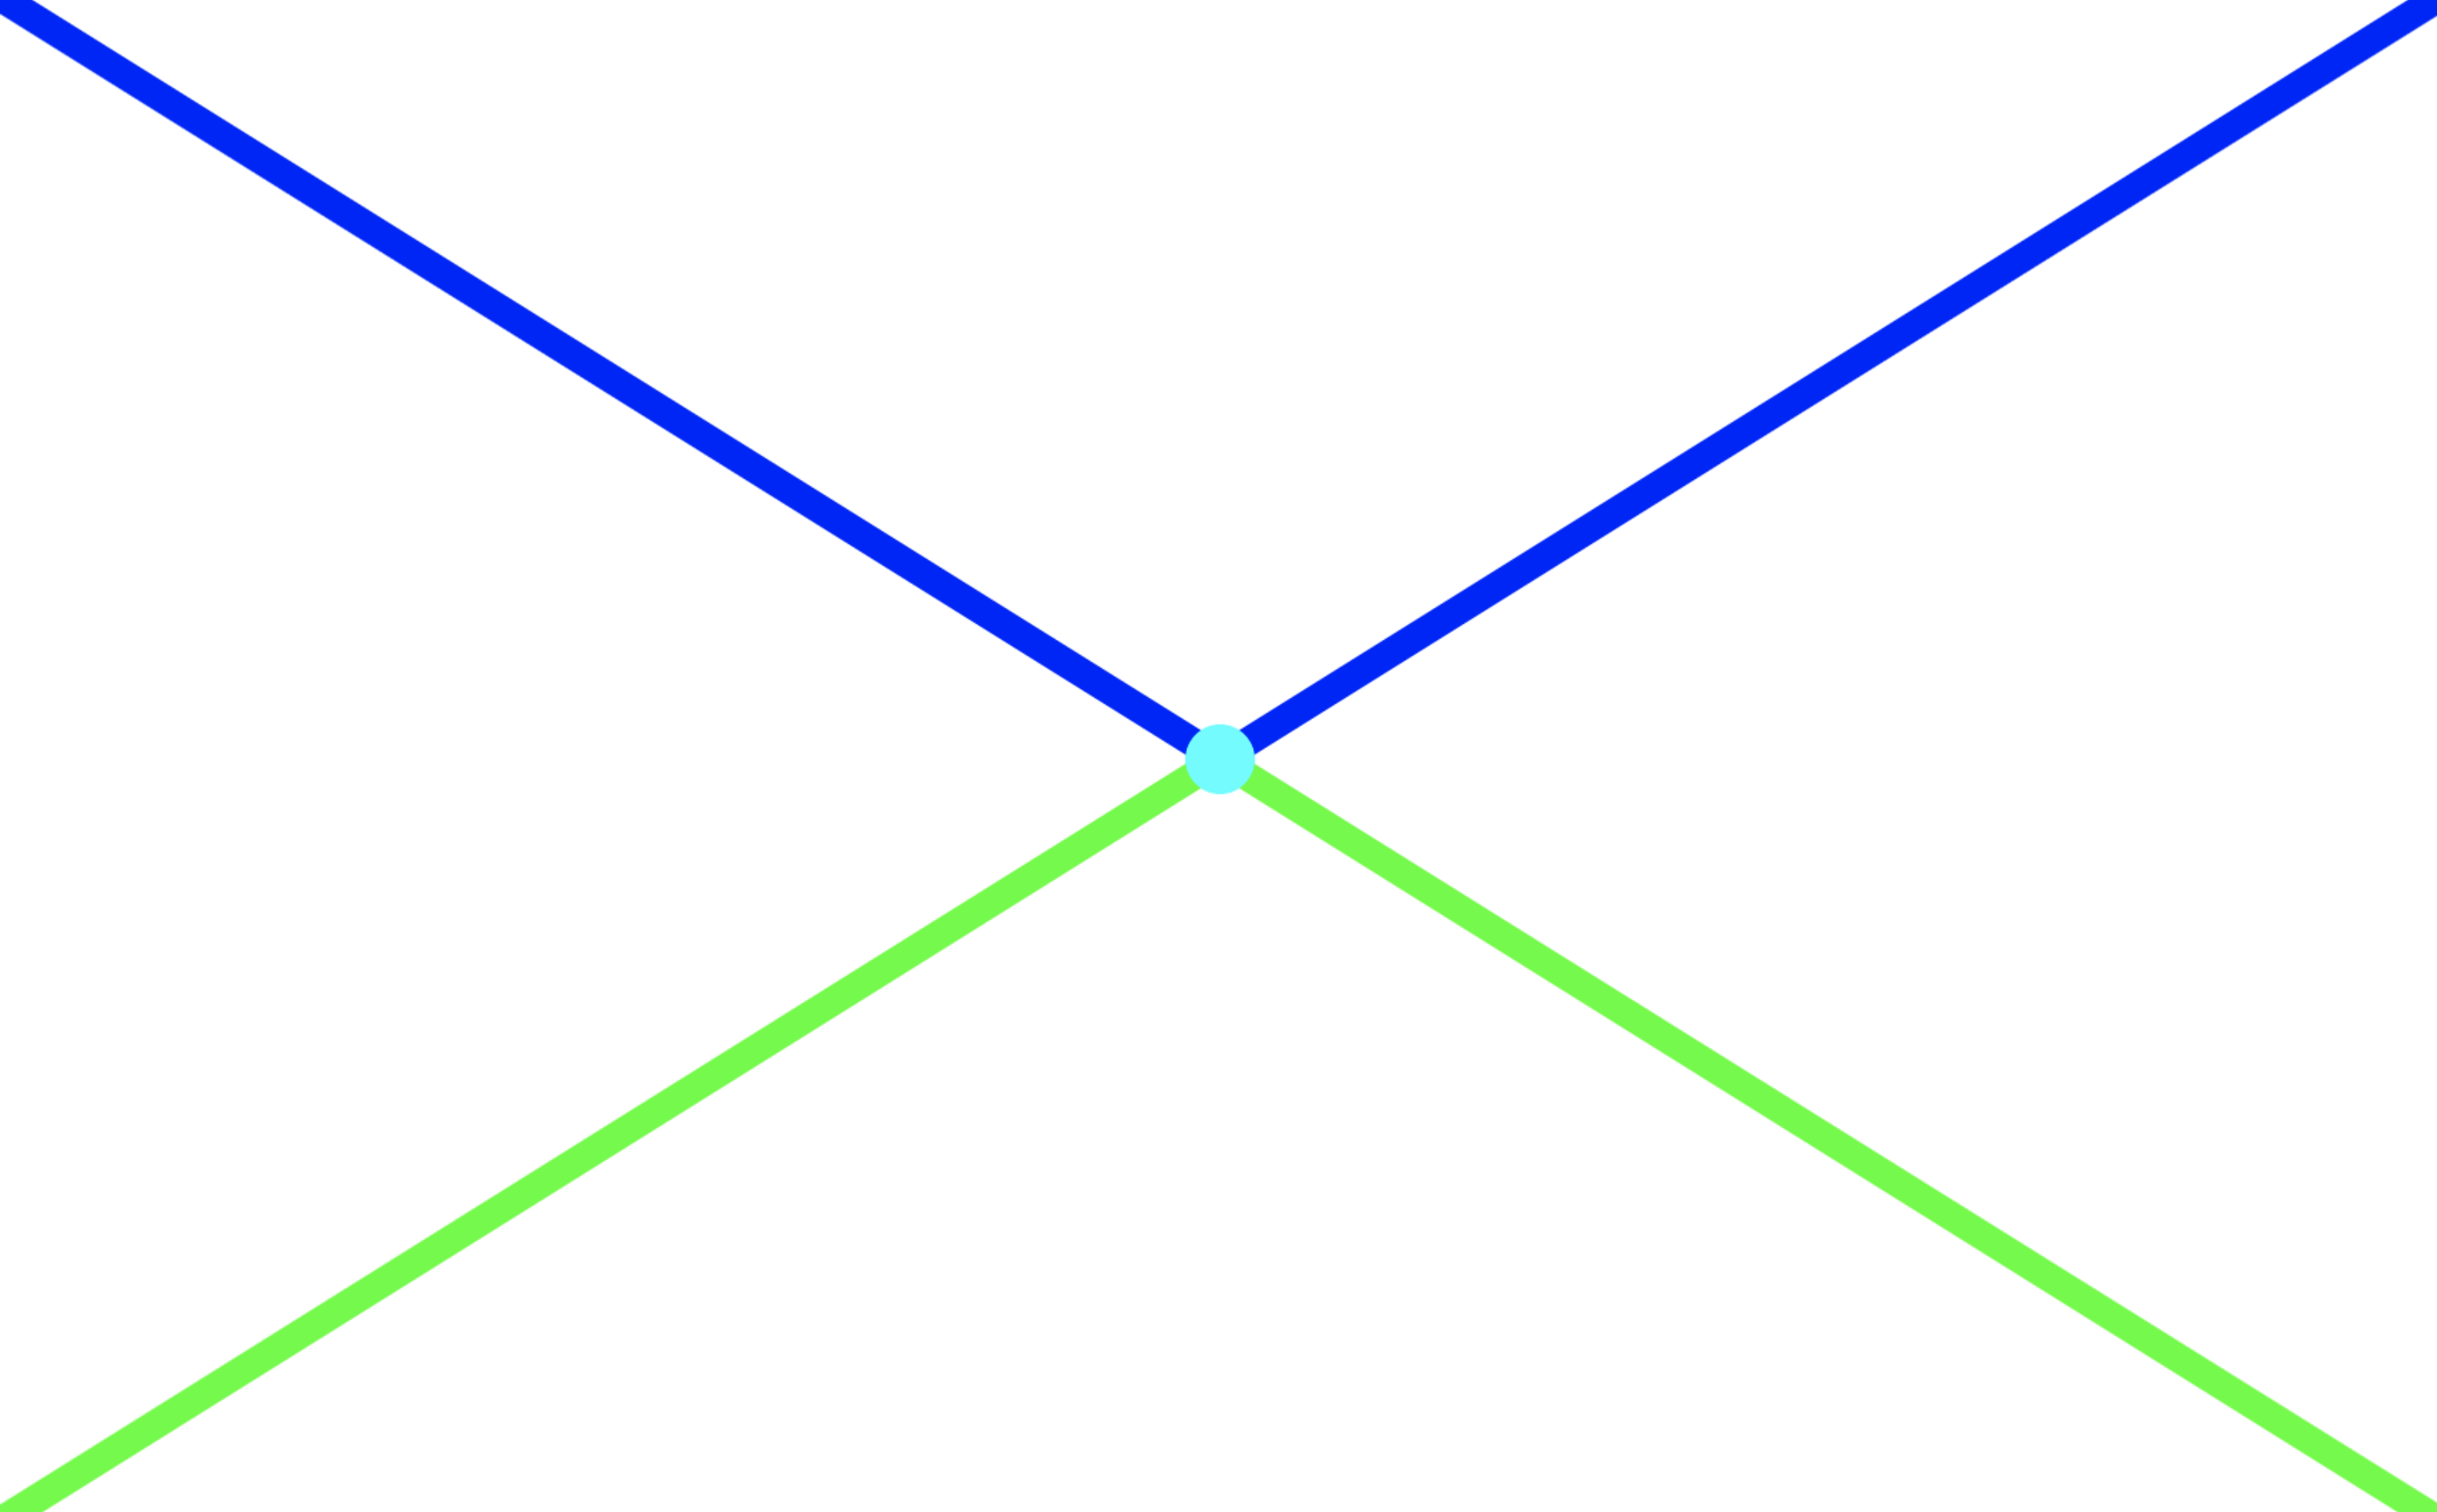
\includegraphics[width=\textwidth]{screen}
	\caption{Nieuwe schermachtergrond}
	\label{fig:screen}
\end{figure}

